\documentclass{beamer}


\usepackage{graphicx}


\author{Damien DELPY}
\title{Implementation of a Self Organizing Map}
\institute{ENSEIRB-MATMECA}


\setbeamertemplate{footline}{%
	\hfill\insertframenumber/\inserttotalframenumber
}


\begin{document}

\begin{frame}
	
	\titlepage
\end{frame}


\begin{frame}

	\tableofcontents[sectionstyle=show,subsectionstyle=show/shaded/hide,subsectionstyle=show/shaded/hide]
\end{frame}



\section{Overview}
	
	\begin{frame}

		\begin{center}
			
			\Huge OVERWIEW
		\end{center}
	\end{frame}


	\begin{frame}{What is a SOM ?}
		
		\begin{block}{Definition}
 
It is a neural network of just one layer : the output layer.
 	
			
		\centering
			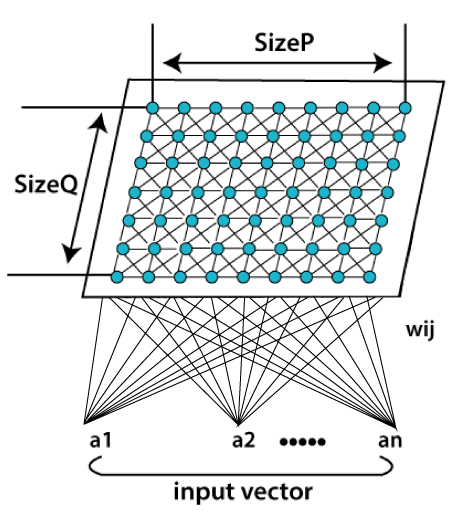
\includegraphics[width=0.3\linewidth]{pics/som_example_diapo_1.png}
		\end{block}		

		\begin{block}{Wikipedia}

A self-organizing map (SOM) is used to produce a low-dimensional (typically two-dimensional) representation of a higher dimensional data set, while preserving the topological structure of the data. 
		\end{block}
	\end{frame}
	
	
	\begin{frame}{Similarities with a Perceptron}

	\end{frame}
	
		
	\begin{frame}{Motivation}
	
	\end{frame}
	
	
	\begin{frame}{Similarities with K-means algorithm}
	
	\end{frame}

	
	\begin{frame}{Convergence}
	
	\end{frame}



\section{Algorithm}

	\begin{frame}
	
		\begin{center}
			
			\Huge ALGORITHM
		\end{center}
	\end{frame}










\section{Bibliography}
	
	\begin{frame}
	
		\begin{center}

			\Huge BIBLIOGRAPHY
		\end{center}
	\end{frame}


	\begin{frame}
	
https://www.baeldung.com/cs/som-algorithm
	\end{frame}





\end{document}
